There are 9 components in our laser harp instrument. These components are referred as subsystems which combine to give definition to the layers discussed above.

The Power System layer consists of single subsystem, Battery. It is main power source for all the components of the instrument. It will be comprised of single or combination of multiple 12V DC batteries. This subsystem will be place in the base of the instrument, will be wired to each component.

The Frames & Component system is comprised of four subsystems Lasers & Receptors, Mister, Touchscreen Display and Speaker. Lasers & Receptors will be combination of multiple laser diodes positioned directly above the photo resistors, which will create laser beams. The interference of laser beams will be detected by the receptors and the resulting signals is sent to MIDI encoder. Mister acts as an individual unit and does not communicate with any other components whereas speakers get its input from the sound card of the sound module layer. There will also be a 6-inch touchscreen display at the front center of the frame. It is used for presets control and adjust sound effects such as gain and reverb.

The MIDI converter layers consists of single component i.e. MIDI encoder. The encoder is likely to be housed in a teensy microcontroller which takes the signals passed on by the receptors and changes it into MIDI signals. Those MIDI signals are forwarded towards MIDI decoder of sound module.

The sound module layer contains three components. MIDI Decoders gets MIDI signals from the MIDI encoder. It interprets those signals, and which is fed into fluidsynth software. It allows the users to manipulate the frequency, depth, dampness, speed, etc. of the incoming signals. The resulting sound is in turn passed onto speakers for audio output via sound card. 


\begin{figure}[h!]
	\centering
 	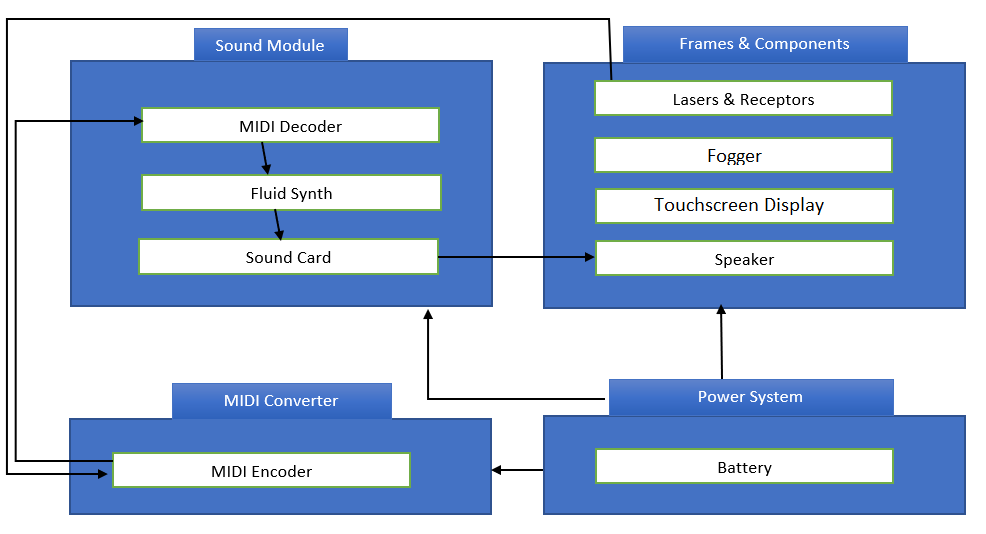
\includegraphics[width=\textwidth]{images/data_flow}
 \caption{A simple data flow diagram}
\end{figure}
